\documentclass{article}

\usepackage[utf8]{inputenc}
\usepackage{amsmath}
\usepackage{amsfonts}
\usepackage{amssymb}
\usepackage{graphicx}
\usepackage[table,xcdraw]{xcolor}
\usepackage[bookmarks,hypertexnames=false,debug,linktocpage=true,hidelinks]{hyperref}
\usepackage{placeins}

\hypersetup{
    colorlinks,
    linktoc=all,
    linkcolor={blue},
    citecolor={blue},
    urlcolor={blue}
}

\usepackage{tikz}
\newcommand*\circled[1]{\tikz[baseline=(char.base)]{
            \node[shape=circle,draw,inner sep=2pt] (char) {#1};}}


\graphicspath{ {./images/} }

\renewcommand{\contentsname}{Indice}

\makeatletter
\newcommand*{\rom}[1]{\expandafter\@slowromancap\romannumeral #1@}
\makeatother

\usepackage[a4paper,top=2cm,bottom=2cm,left=2cm,right=2cm]{geometry}

\setcounter{section}{-1}

\title{\textbf{\Huge Analisi dei Requisiti}}
\author{Matteo Girardi, Vasile Donmovil, Timeskipper \\ Gruppo T45 - Deliverable D1}
\date{2022}

\begin{document}

\maketitle

\clearpage
\tableofcontents
\clearpage

\section{Scopo del documento}
\begin{description}
    \item[] Il presente documento illustra le diverse caratteristiche del sistema software da realizzare, chiamato \textit{Bloodstream}. L’obittetivo del progetto è la realizzazione di una piattaforma (web app) che permetta di gestire prenotazioni per la donazione di sangue presso l’Associazione Volontari Italiani del Sangue.
    \item[] Verranno analizzati gli obiettivi del progetto, definiti i requisiti funzionali e non funzionali e infine verranno esposti i requisiti di front-end e di back-end.
    \item[] Il documento analizza i seguenti aspetti:
    	\begin{itemize}
    	\item Obiettivi del progetto
    	\item Requisiti Funzionali
    	\item Requisiti non Funzionali
    	\item Requisiti del Front-End
    	\item Requisiti del Back-End
    	\end{itemize}
\end{description}
\clearpage

\section{Obiettivi del progetto}
\begin{description}
    \item[] Il progetto ha come obiettivo la realizzazione di una piattaforma in grado di facilitare l'organizzazione delle sessioni di prelievo del sangue a cui partecipano i donatori. \\
    Tale soluzione software sarà una webapp, accessibile quindi da qualunque dispositivo in grado di accedere ad Internet.
    
    \item[] Dal punto di vista dell'utente:
        \begin{itemize}
            \item Sarà possibile consultare una pagina web dove vengono mostrate le date disponibili e le stanze in cui avvengono i prelievi.
            \item Sarà possibile prenotare le sessioni di prelievo.
            \item Tutte le prenotazioni saranno raggruppate in una zona dedicata della piattaforma, in quella che si può definire "Area Riservata".
            \item Una volta recato in struttura il donatore potrà  accedere alla sala da lui prenotata provvisto di codice di prenotazione, entro la scadenza prefissata.
        \end{itemize}
\end{description}
\clearpage


\section{Requisiti}
\begin{description}
	\item[] Si individuano 3 tipi di utenti che interagiranno con la webapp:
		\begin{itemize}
		\item \circled{Un} Utente Non Registrato
		\item \circled{Re} Utente Registrato
		\item \circled{Ad} Utente Amministratore
		\end{itemize}
	\item Ciascun utente avrà privilegi differenti e relativi requisiti. Di seguito vengono elencati i requisiti funzionali.
\end{description}

\subsection{Requisiti Funzionali}
\renewcommand\thesubsubsection{RF\arabic{subsubsection}}
\subsubsection{Visualizzazione Date} \label{rf_1}
\begin{description}
    \item[] L'utente può visualizzare tramite un calendario i giorni in cui è disponibile una o più sale.
    \item Questo requisito appartiene a: \circled{Un} \circled{Re} \circled{Ad}
\end{description}

\subsubsection{Prenotazione Sala} \label{rf_2}
\begin{description}
    \item[] L'utente può effettuare una prenotazione per una sala, scegliendo tra quelle disponibili in un dato giorno tramite un calendario aggiornato.
    \item Questo requisito appartiene a: \circled{Re}
\end{description}

\subsubsection{Gestione prenotazioni} \label{rf_3}
\begin{description}
    \item[] I donatori registrati potranno consultare le proprie prenotazioni imminenti e passate.
    \item Questo requisito appartiene a: \circled{Re} \circled{Ad}
\end{description}

\subsubsection{Annullare una Prenotazione} \label{rf_4}
\begin{description}
    \item[] L'utente può revocare la propria prenotazione, con il vincolo di poterlo fare sino a 24 ore precedenti all'ora prefissata durante la fase di prenotazione.
    \item Questo requisito appartiene a: \circled{Re} \circled{Ad}
\end{description}

\subsubsection{Login} \label{rf_5}
\begin{description}
    \item[] L'utente può accedere al servizio, autenticandosi con codice fiscale e codice OTP.
    \item Questo requisito appartiene a: \circled{Re} \circled{Ad}
\end{description}

\subsubsection{Logout} \label{rf_6}
\begin{description}
    \item[] L'utente registrato può disconnettersi dalla sessione.
    \item Questo requisito appartiene a: \circled{Re} \circled{Ad}
\end{description}

\subsubsection{Creazione Nuovo Account} \label{rf_7}
\begin{description}
    \item[] L'utente amministratore può aggiungere manualmente un nuovo account donatore alla piattaforma.
    \item Questo requisito appartiene a: \circled{Ad}
\end{description}

\subsubsection{Gestione Account} \label{rf_8}
\begin{description}
    \item[] I donatori registrati potranno gestire il proprio account aggiornando le proprie informazioni personali.
    \item Questo requisito appartiene a: \circled{Re} \circled{Ad}
\end{description}

\subsubsection{Rimozione Account} \label{rf_9}
\begin{description}
    \item[] I donatori registrati potranno scegliere di cancellare il proprio account.
    \item Questo requisito appartiene a: \circled{Re} \circled{Ad}
\end{description}

\subsubsection{Modifica Stato Sala} \label{rf_10}
\begin{description}
    \item[] L'utente amministratore può modificare lo stato di una specifica sala. Sarà permesso tramite un’apposito pannello di controllo aggiungere nuovi slot
disponibili oppure eliminare quelli esistenti (indipendentemente dalla disponibilità di quest’ultimo).
    \item Questo requisito appartiene a: \circled{Ad}
\end{description}

\subsubsection{Notifica Prenotazione} \label{rf_11}
\begin{description}
    \item[] L'utente donatore riceve una notifica via SMS e/o Email che lo informa dell'imminente sessione di donazione.
    \item Questo requisito appartiene a: \circled{Re}
\end{description}

\clearpage
\subsection{Requisiti non Funzionali}
\renewcommand\thesubsubsection{RNF\arabic{subsubsection}}
\subsubsection{Privacy} \label{rnf_1}
\begin{description}
    \item[] L’applicazione deve essere progettata e realizzata in ottemperanza alle vigenti disposizioni di legge in materia di
tutela della privacy e trattamento dei dati, nello specifico anche al Regolamento Europeo per la protezione
dei dati (GDPR).
L’applicazione non permetterà ai suoi operatori di conoscere alcuna informazione personale (a esclusione del
DPO) sui clienti, eccetto il nome utente
\end{description}

\subsubsection{Sicurezza} \label{rnf_2}
\begin{description}
    \item[] Per garantire la sicurezza di chi utilizza il servizio, ogni utente avrà solamente accesso ai suoi dati personali, non potrà accedere a quelli altrui, cosicchè le informazioni rimangano riservate.
 Il flusso di dati opererà sotto protocolli di elevata sicurezza, criptando il traffico.
Ci si affida a servizi terzi per la protezione del servizio da attacchi mirati e tentativi di hacking malevoli.
Verranno impiegate le più adeguate contromisure per garantire la sicurezza degli utenti, al fine di fornire un prodotto sicuro.
\end{description}

\subsubsection{Scalabilità} \label{rnf_3}
\begin{description}
    \item[] La piattaforma viene progettata sfruttando tecnologie che facilitino l'elaborazione di un numero sempre crescente di utenti, in maniera efficace. Il servizio deve appunto garantire l'operatività ad un numero di utenti variabile.
\end{description}


\subsubsection{Affidabilità} \label{rnf_4}
\begin{description}
    \item[] Il sistema di trasmissione dovrà garantire la più alta affidabilità possibile. Pertanto verranno adottate
logiche di re-invio per le operazioni di trasmissione tra i vari livelli coinvolti, puntando a ridurre al minimo la mancata trasmissione dei dati.
\end{description}

\subsubsection{Resilienza} \label{rnf_5}
\begin{description}
    \item[] Il sistema disporrà di sistemi di ridondanza in grado di garantire l'operatività anche durante episodi di parziale disservizio di componenti interne.
\end{description}

\subsubsection{Accessibilità} \label{rnf_6}
\begin{description}
    \item[] Il servizio sarà offerto tramite un portale web, quindi fruibile da ogni dispositivo in grado di mostrare correttamente una pagina web. La web app dovrà essere accessibile sui più grandi e famosi browser senza compromettere nè l’esperienza di navigazione nè la sicurezza dell'utente.
\end{description}

\subsubsection{Monitoraggio} \label{rnf_7}
\begin{description}
    \item[] La piattaforma prevede un sistema che registra, salva e analizza gli accessi e gli eventi che avvengono, disponendoli in maniera comprensibile.
\end{description}

\subsubsection{Multi-lingua} \label{rnf_8}
\begin{description}
    \item[] Il servizio sarà offerto in due lingue (Italiano e Inglese).
\end{description}

\clearpage
\section{Front-End}

\subsection{Homepage}
\begin{figure}[htp]
\centering
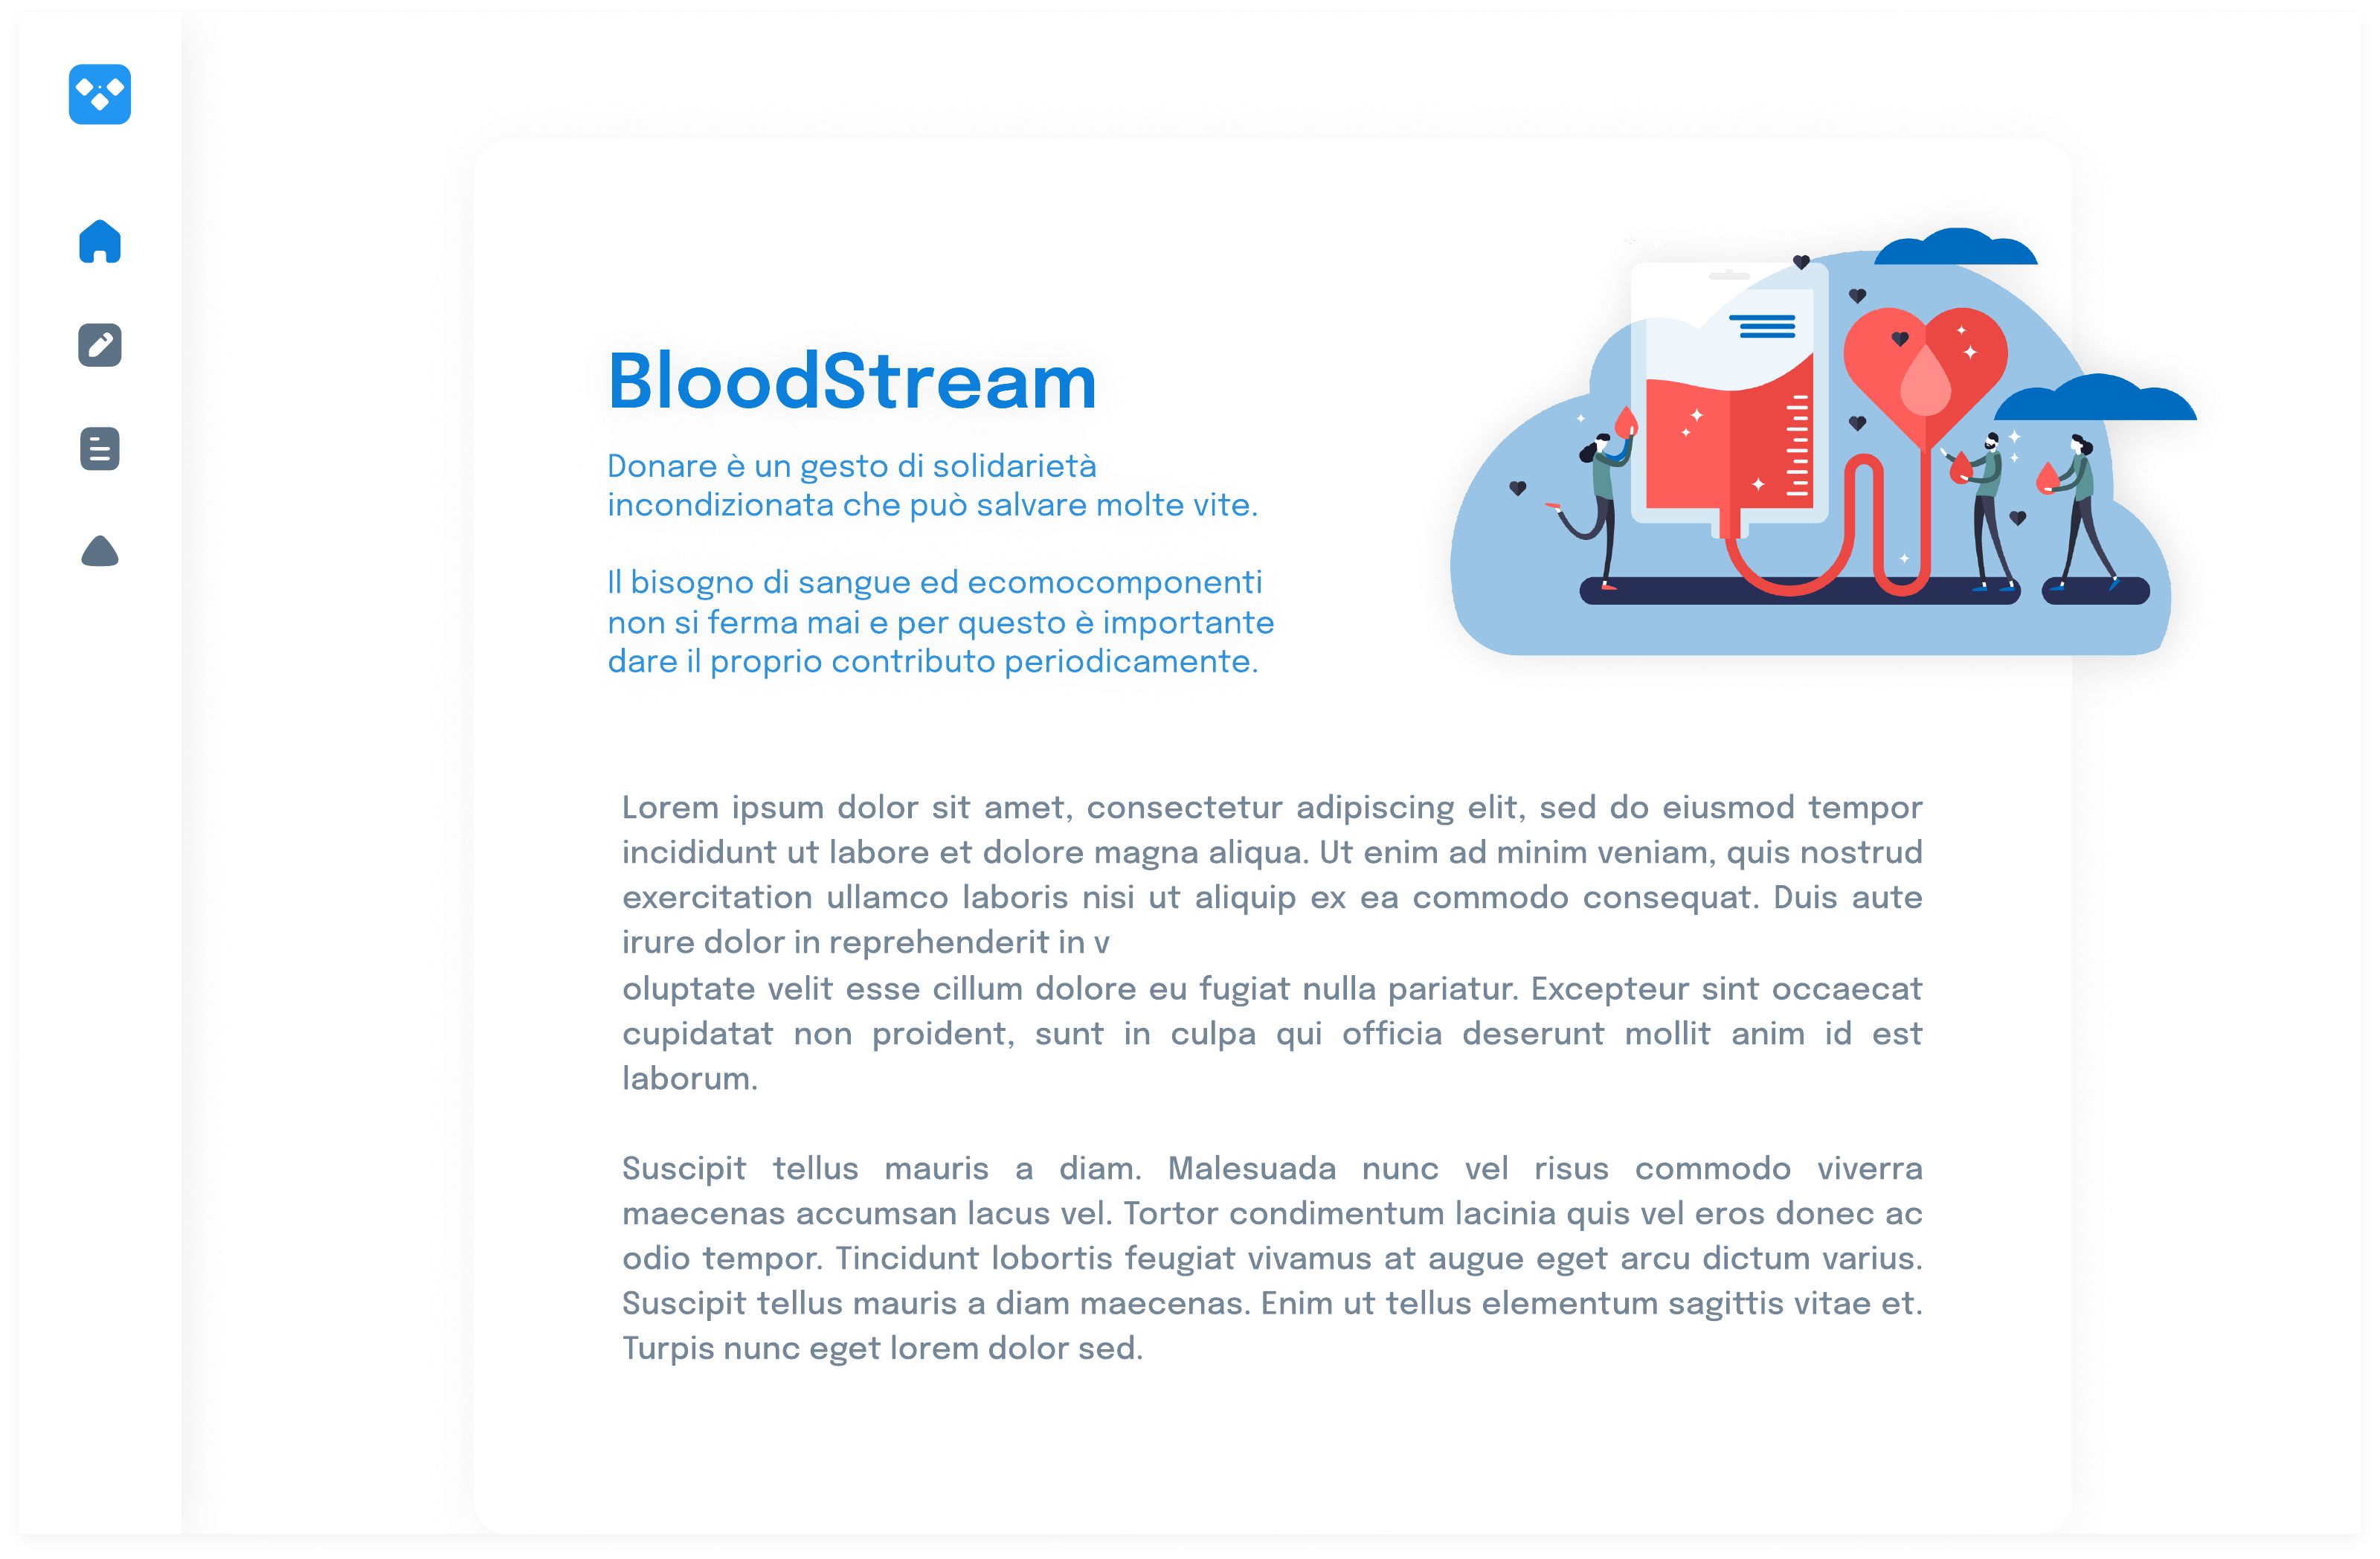
\includegraphics[width=\textwidth,height=\textheight,keepaspectratio]{media/bloodUI-1.png}
\caption{Pagina principale}
\end{figure}

\FloatBarrier

\clearpage
\subsection{Login}
\begin{figure}[htp]
\centering
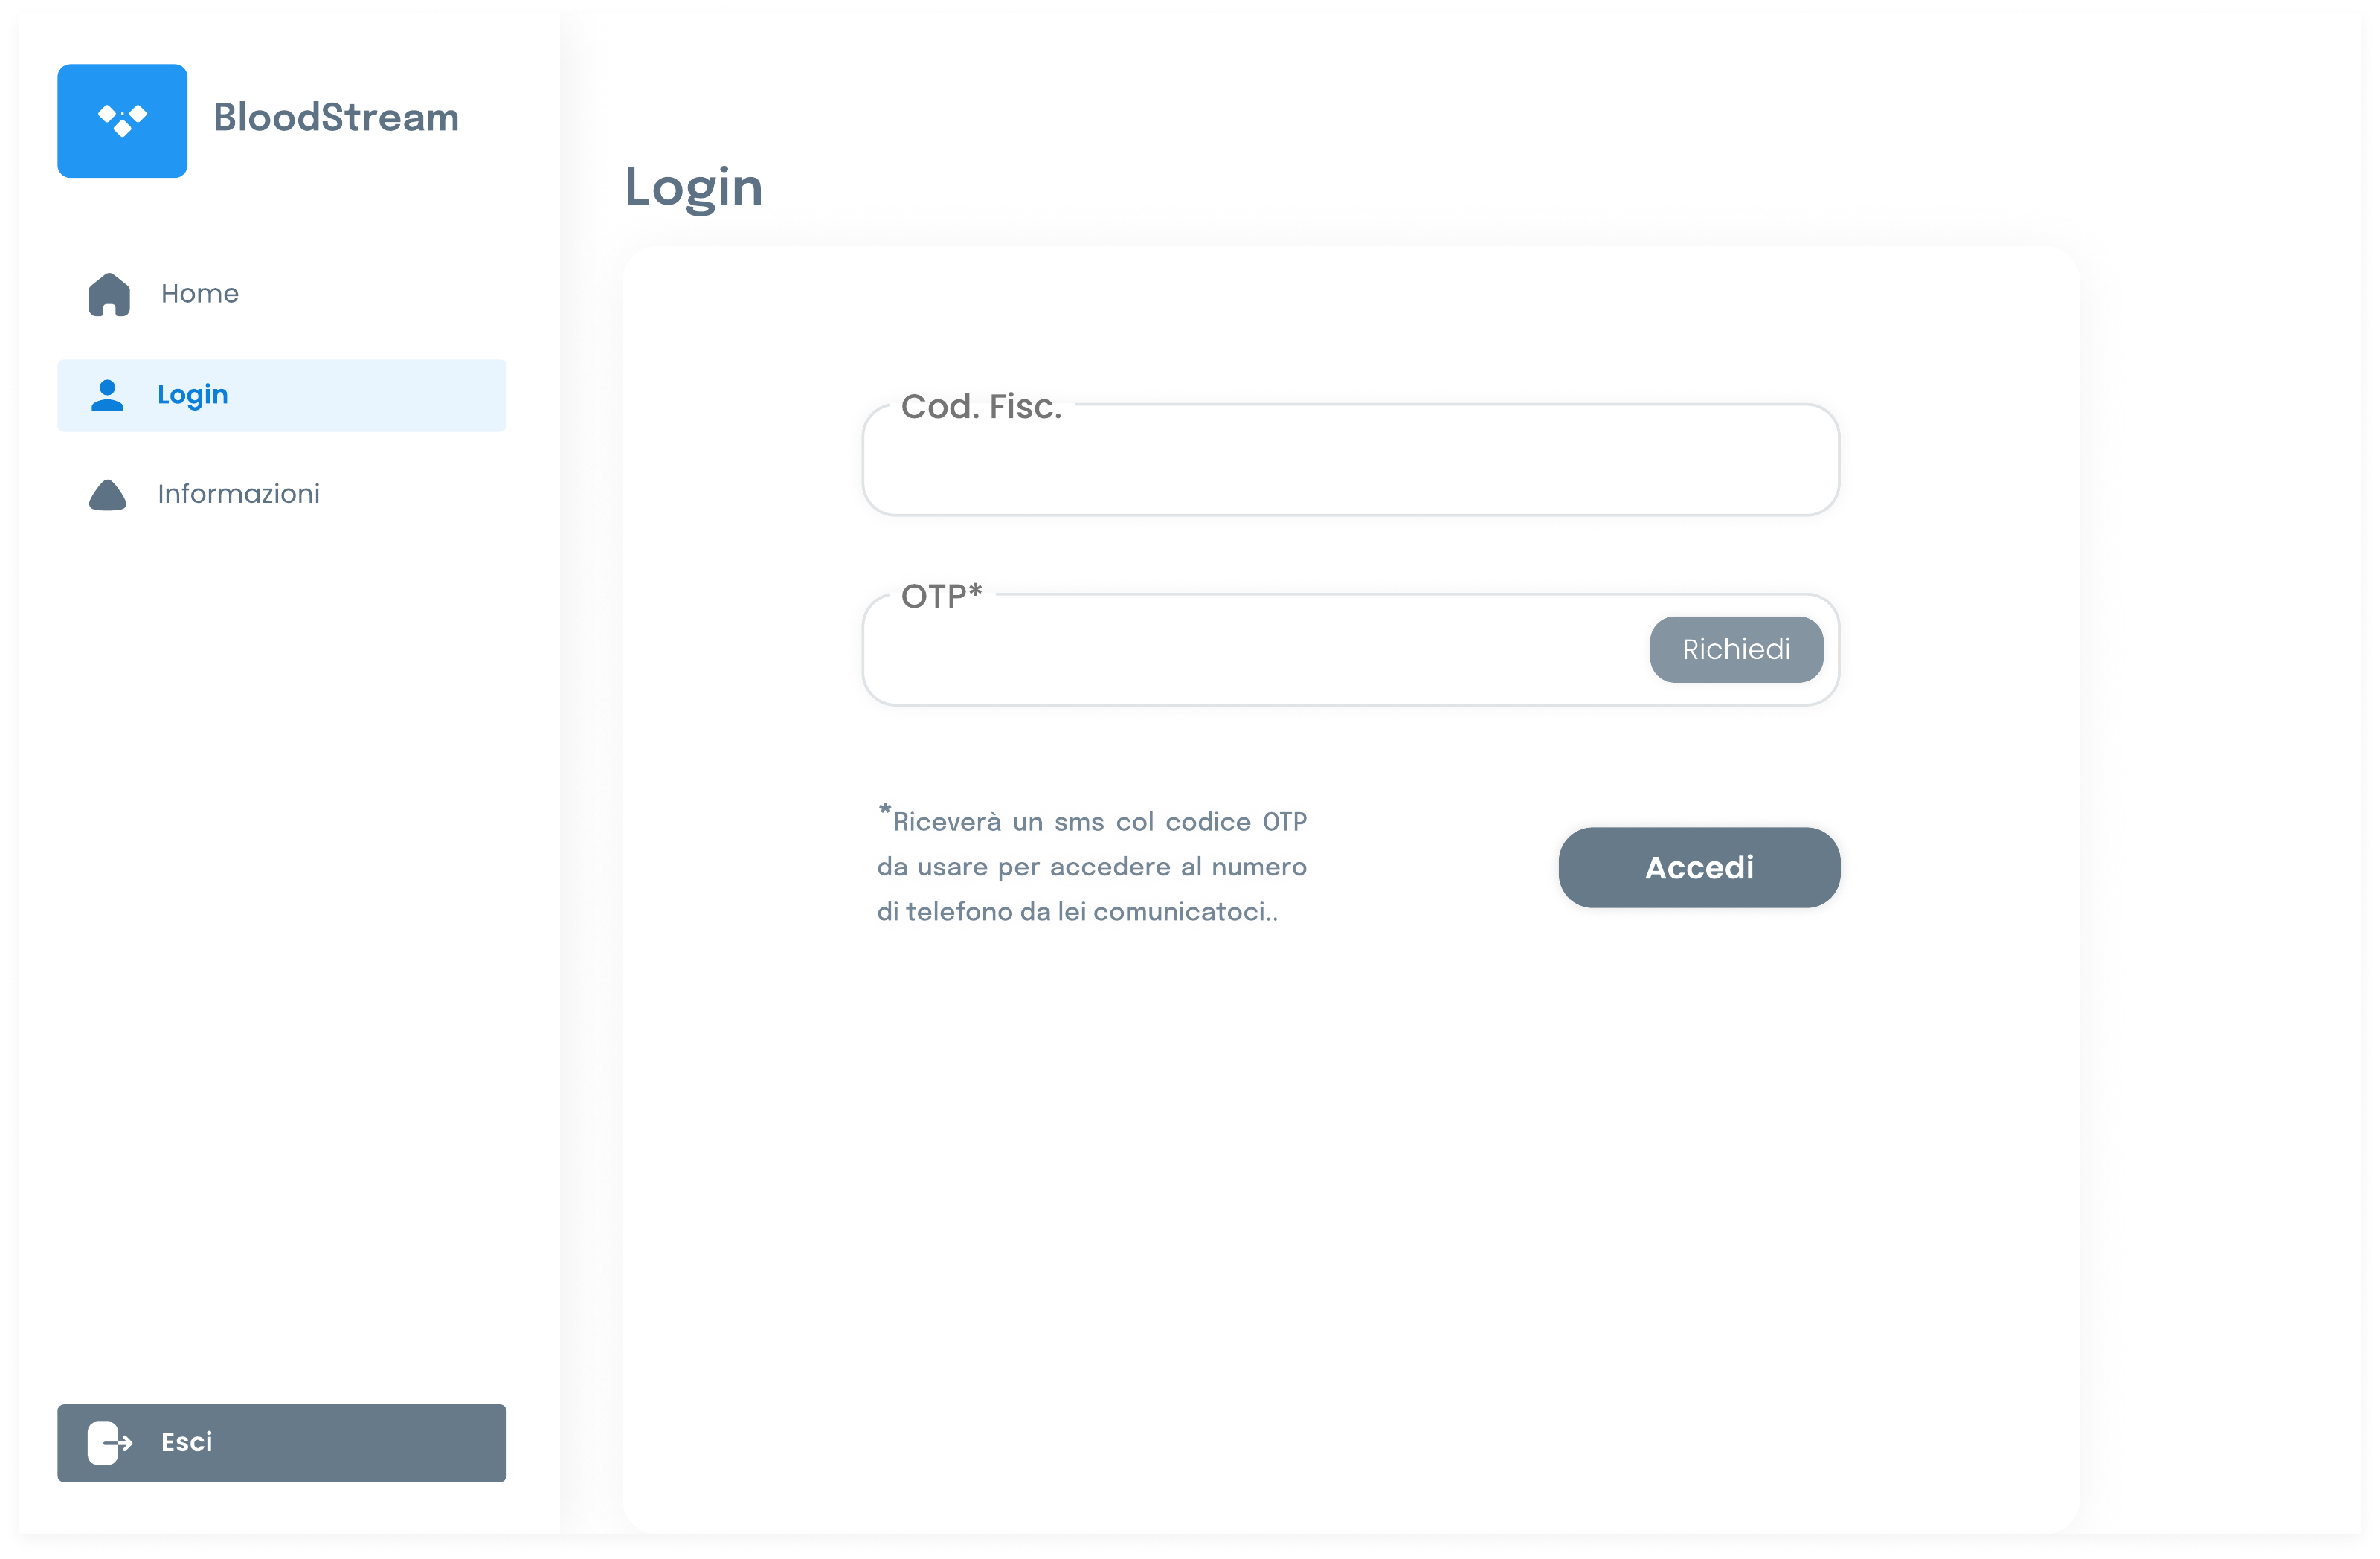
\includegraphics[width=\textwidth,height=\textheight,keepaspectratio]{media/bloodUI-4.png}
\caption{Schermata di Login}
\end{figure}

\FloatBarrier

\clearpage
\subsection{Calendario}
\begin{figure}[htp]
\centering
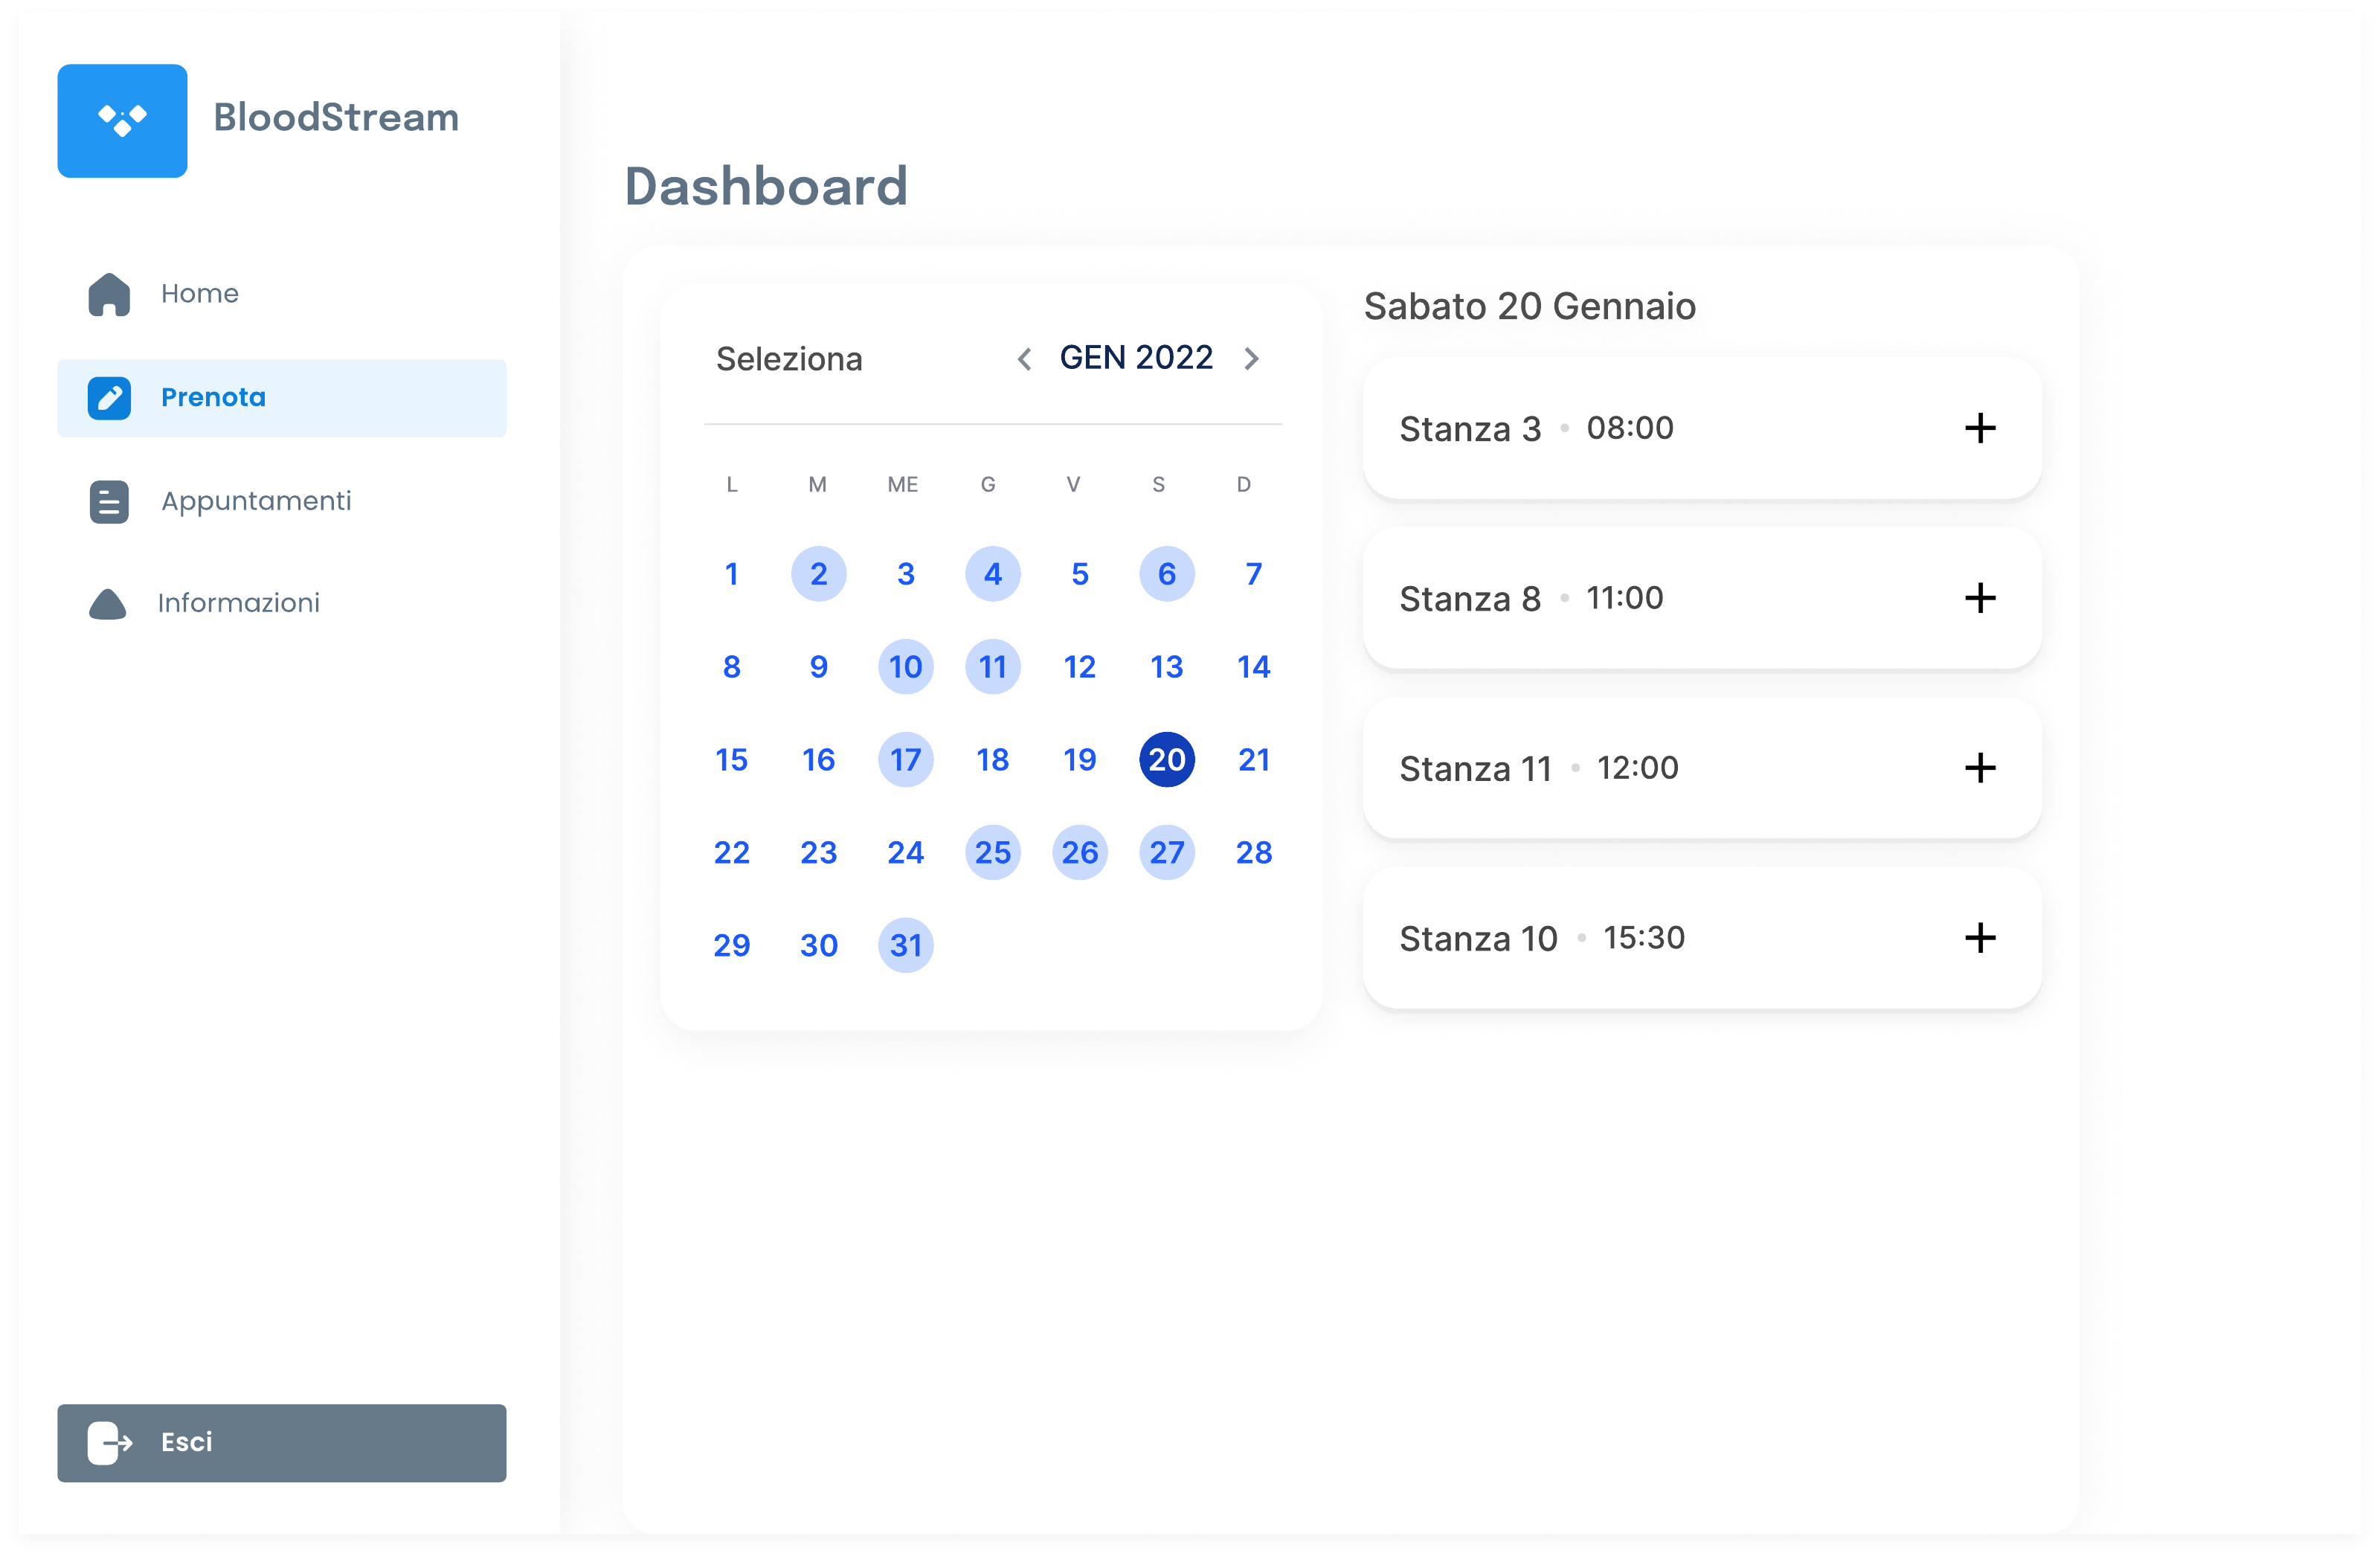
\includegraphics[width=\textwidth,height=\textheight,keepaspectratio]{media/bloodUI-2.png}
\caption{Calendario prenotazioni}
\end{figure}

\FloatBarrier

\clearpage
\subsection{Area Privata}
\begin{figure}[htp]
\centering
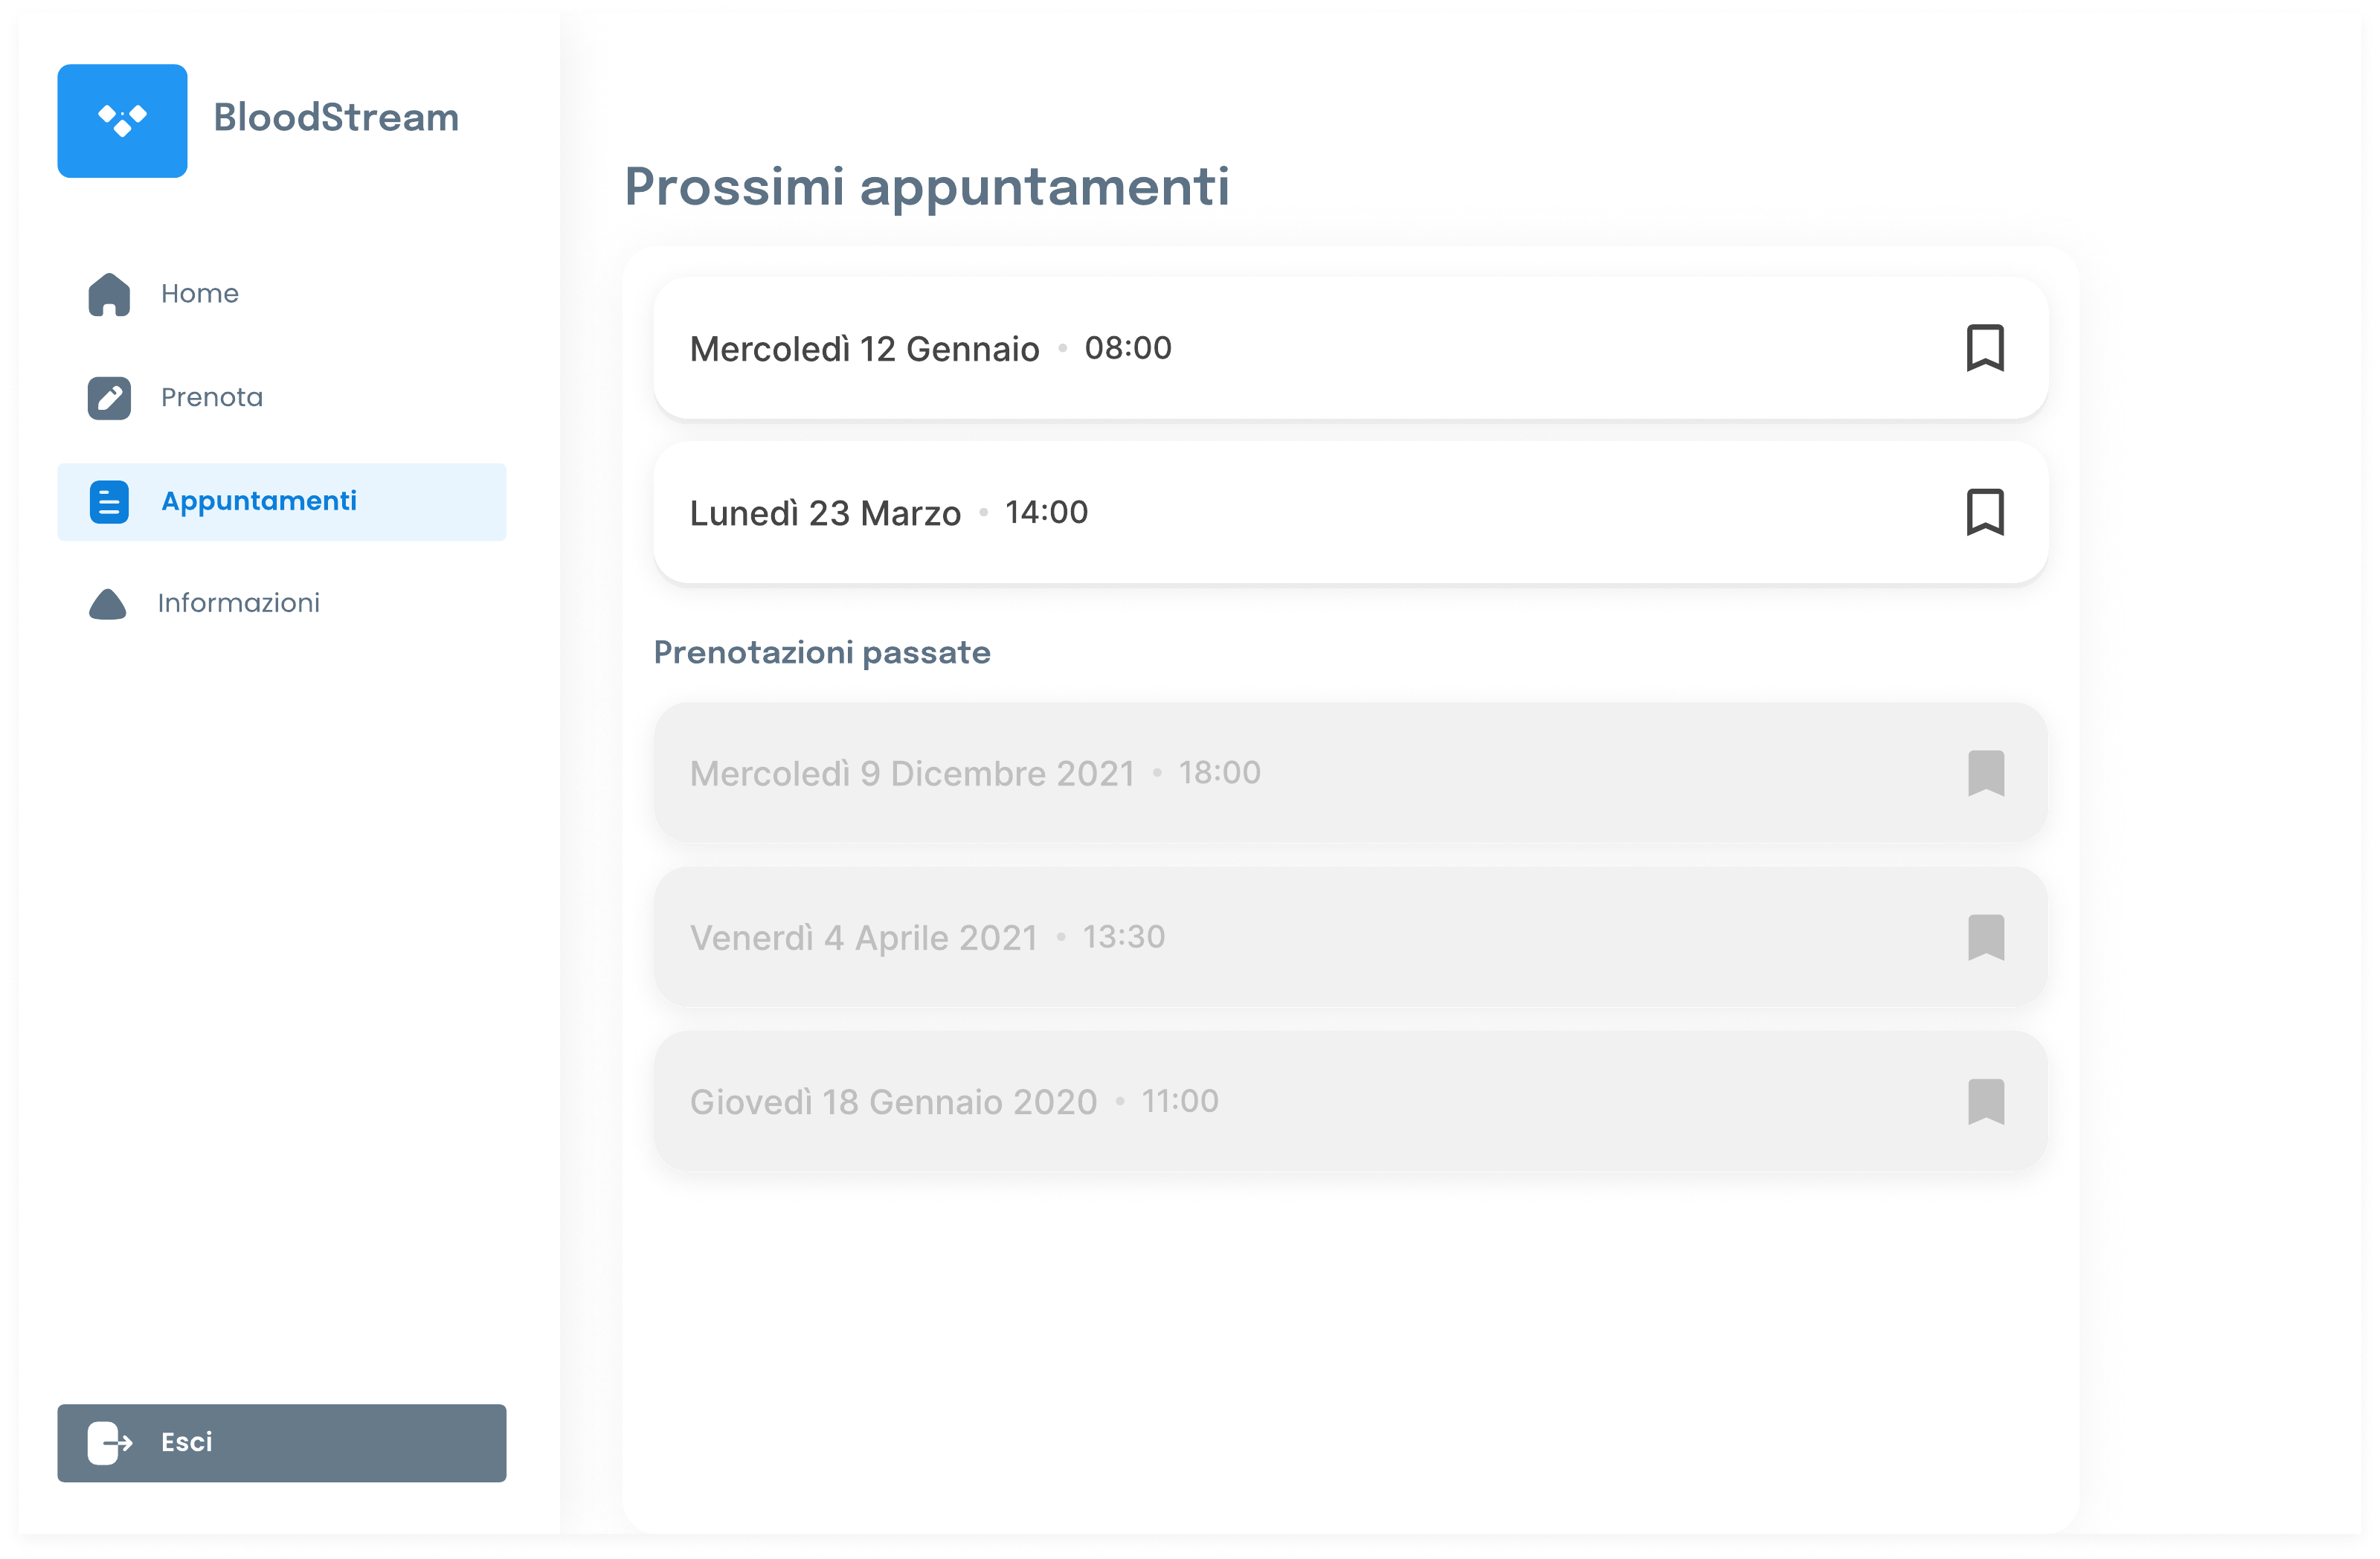
\includegraphics[width=\textwidth,height=\textheight,keepaspectratio]{media/bloodUI-3.png}
\caption{Area riservata}
\end{figure}

\FloatBarrier

\clearpage
\section{Back-End}
\begin{description}
    \item[] La piattaforma oltre ad interfacciarsi con l’utente si interfaccia anche con CloudFlare e col suo sistema
    di “reverse proxy”; inoltre le risorse statiche del sito, come le immagini, verrano salvate nella cache di Cloudflare.
    L’invio di SMS sarà gestito tramite le api di Twilio, azienda leader del settore, mentre l'invio automatico di Email avverà grazie a un server mail esterno.
    \\ Qui in seguito viene fornito uno schema logico servizi con i quali l’applicazione interagisce:

\end{description}

\begin{figure}[htp]
    \centering
    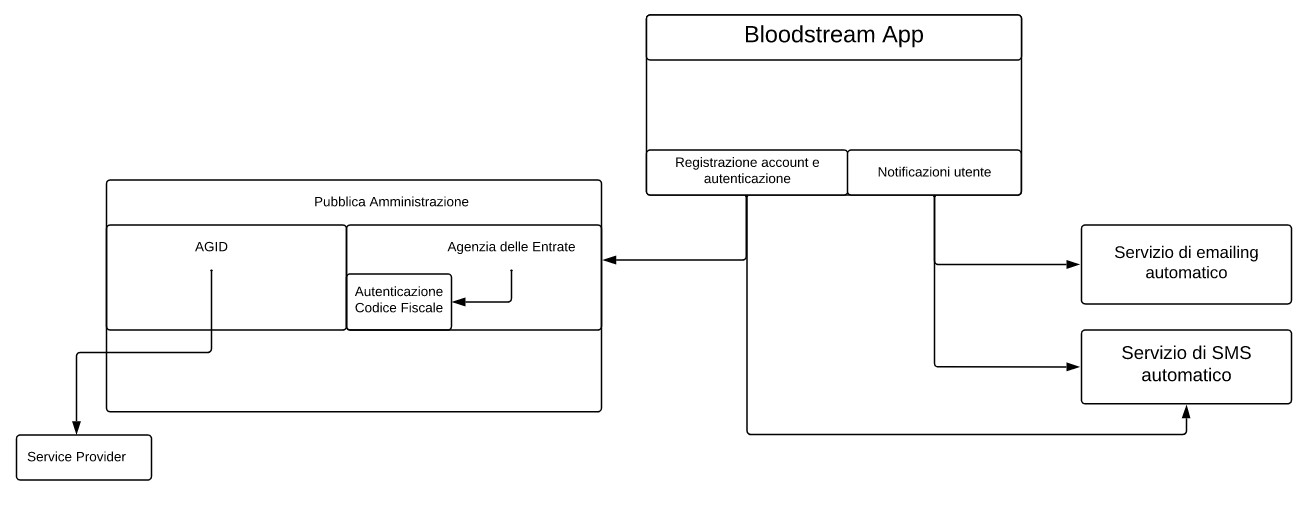
\includegraphics[width=\textwidth,height=\textheight,keepaspectratio]{media/schema-backend.png}
    \caption{Schema backend}
\end{figure}


\end{document}